

The proposed autoscaling system scales a web application in respose to change in throughput at fixed intervals, which we denote by reconfiguration intervals of 15 minutes. This architecture has the following key components:

\noindent\textbf{Predictor: } Predictor component takes the monitoring data as input and uses different time-series analysis techniques to predict the future service demand for the next time interval. 

\noindent\textbf{Profiler: } This component measures the current and maximum capacity of each type of provisioned vm instance. To do that, the Profiler uses online profiling techniques without any server instrumentation.

\noindent\textbf{Dynamic load balancer: } In order to adapt our system to the heterogeneity of cloud platforms, this component dynamically assign weights to the backend servers to proportionally distribute the incomming traffic across them taking into account the heterogeneity of their performance characteristics.


\noindent\textbf{Scaler: }  This component contains the central intelligence of our autoscaling system. Scaler uses the Predictor and Profiler components to find the optimal provisioning strategy that fulfills a pre-established SLO (Service Level Objective). Furthermore, this component constantly analyzes the behaviour of the provisioned VMes to trigger the Dynamic load balancer component.

\begin{figure}[htb]
  \begin{center}
    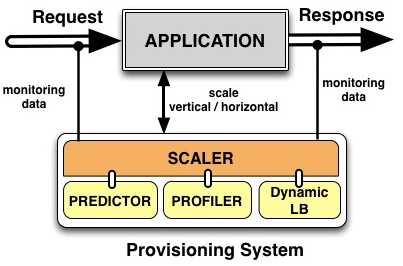
\includegraphics[width=.85\linewidth]{images/monitoringSchema}
  \end{center}
\vspace{-5mm}
  \caption{Auto-scaling system.}
  \label{autoScalingSys}
\end{figure}

\subsection{Predicting future service demand}
There is a vast literature related to resource provisioning systems that utilizes time-series analysis to predict the future service demand. However, it is not clear which prediction technique to employ when having a very heterogeneous workload mix. 

As a consequence, we designed a Predictor component that first analyzes the monitoring data using five different prediction techniques (six very soon), and then uses the model that exhibits the lowest cumulative error measure at any given moment (previous iteration). To handle different types of workload, the Predictor component utilizes the following statistical  and learning-based techniques for estimating the future service demand:

\begin{itemize}
\item Linear Regression (LR): It is a statistical method whose objective consists to find a polynomial function on which the distance from each of the points to a polynomial curve is the smallest as possible. This model is applied to time-series with a linear trend. Equation ...

\begin{equation}\label{xx}
\begin{split}
Y = {\beta}_1 +  \sum_{i=1}^n {\beta}_i x_i 
\end{split}
\end{equation}

\item Exponential Smoothing (ES): Regarding the different variety of exponential smoothing methods, we decided to use the \emph{Holt-Winters'} model that can be used for time-series with an existing trend and seasonality. This model fits to daily and seasonal behavior of web applications by assigning weigths over time based on the influence of a smotthing factor \emph{$\alpha$} to the historic data. Equation ..

\begin{equation}\label{xx}
\begin{split}
Y_{t+m} = (2y_t - y_t) + m(y_t - y_t) \alpha / (1 - \alpha) 
\end{split}
\end{equation}

\item Autoregression (AR): Based on the linear regression method, this model defines a polynomial function that first calculates and then uses the auto-correlation coefficients of the time-series similar to finally apply the linear regression model. Equation ...

\begin{equation}\label{xx}
\begin{split}
Y_t =a_1 Y_t-1 + ... + a_p Y_t-p 
\end{split}
\end{equation}


\item Vector Autoregression (VAR): This model is a natural extension of the  autoregressive model to dynamic multivariate time series. The VAR model has proven to be especially useful for describing the dynamic behavior of economic and financial time series and for forecasting. Equation ...

\begin{equation}\label{xx}
\begin{split}
Y_{t} =a_1 Y_{t-1} + ... + a_p Y_{t-p} + {\epsilon}_p
\end{split}
\end{equation}


\item Auto Regression Moving Average (ARMA): This averaging method combines both autoregression and moving average. Equation ...

\begin{equation}\label{xx}
\begin{split}
Y_{t+1} =a_1 Y_{t-1} + a_2 Y_{t-2} + ... + b_o X_t + b_1 X_{t-1} + ...
\end{split}
\end{equation}


\item Neural networks (NN): ...
\end{itemize}


In this system, the Predictor component forecasts the future response time values (5min ahead) of an application answering to the question "When to provision?". These prediction models are fed using the monitoring data collected from the web proxy servers. Furthermore, this component also predicts the future values (1h ahead) of monitoring metrics such as request rate and CPU usage to  identify the resource requirements for the next time intervals. This last prediction will contribute to answer the question "How much to provision?", as mentioned in Section~\ref{profiling}.
When using the Predictor for this purpose, a reduction in the finnacial cost is caused, as offline training phases are not needed to provide accurate predictions to handle a future service demand.

\begin{figure}[htb]
  \begin{center}
    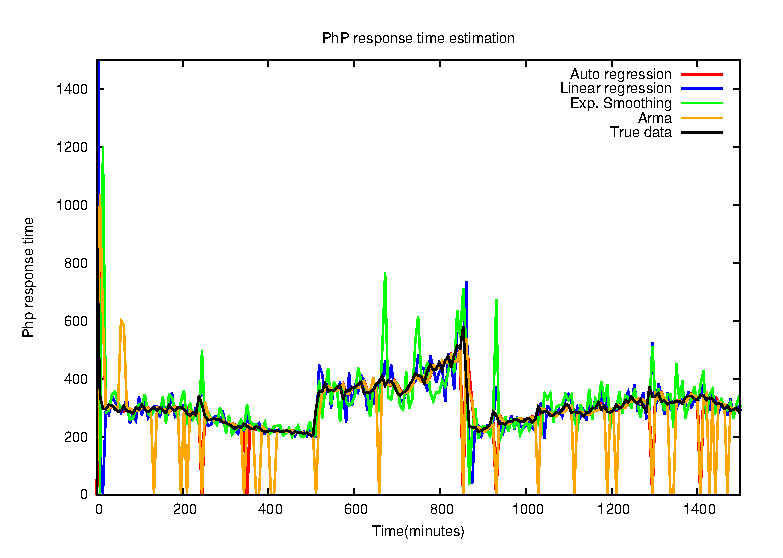
\includegraphics[width=.85\linewidth]{images/prediction_models_6min.eps}
  \end{center}
\vspace{-5mm}
  \caption{Prediction results, response time 5min ahead.}
  \label{threshold}
\end{figure}

To calculate the cumulative error, we use MAPE method  (Moving Average Percentage Errors).

\subsection{Online profiling \label{profiling}}

Regarding the resource heterogeneity of cloud infrastructures, online profiling-based techniques~\cite{kaviani_profiling-as--service:_2011} have recently emerged as a possible solution to the estimation of the resource throughput under certain workload. This technique replicates at runtime a server hosting an application, with a new server with profiling instrumentation. Despite the use of the online-profiling is still under study, the configuration of a parallel environment and the limited accuracy of its scaling decisions are the major drawbacks for its adoption.

In our system, we designed a novel online profiling technique that gives an estimation of the maximum throughput of each allocated vm instance without need for additional resources. To do that, the Profiler component stores the latest hour of monitoring data from each instance's type allocated in one application. The profiling data is composed of monitoring metrics such as the request rate, cpu usage and response time. 

Once the Scaler component decides to trigger a scaling action, the Profiler component processes the profiling data to estimate the resource throughput according the following steps:

\begin{enumerate}
\item Collect the profiling data of each instance's type.
\item Perform a smoothing technique over the profiling data to remove the noise generated by traffic spikes. As illustrated in Figure~\ref{fig:vm_performance}, the Profiler extracts the smoothed 75th and 25th percentiles to identify the maximum-ideal  throughput of each instance while enforcing the performance requirements and avoiding CPU saturation (based on the Amazon EC2 recommendation 30 < CPU usage < 75  ).

\begin{figure*}[htb]
	\begin{minipage}[b]{0.45\linewidth}
		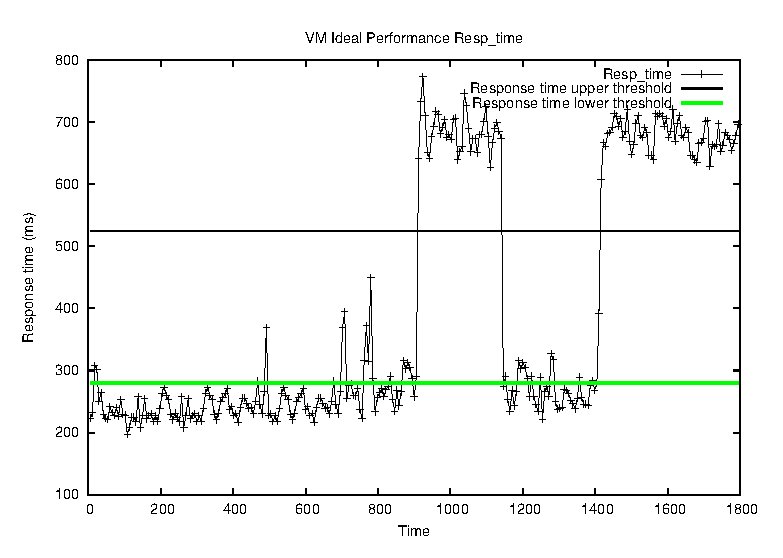
\includegraphics[height=4.5cm]{images/vm_performance_resp.eps}
		\vspace{-4mm}
	\end{minipage}
	\hfill
	\begin{minipage}[b]{0.45\linewidth}
		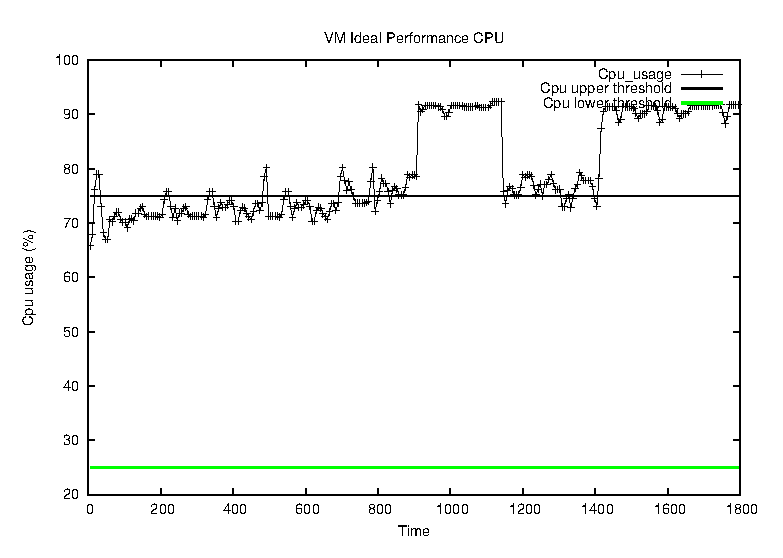
\includegraphics[height=4.5cm]{images/vm_performance_cpu.eps}
		\vspace{-4mm}
	\end{minipage}
\caption{Profiling data and percentiles for the Response time and CPU usage.}
\label{fig:vm_performance}
\end{figure*}


\item Classify the different instance types depending on the performance capacity. The Predictor calculates a factor, named \emph{CPU speed}, as the number of clocks required to process a request (clocks/request) by using the next Equation~\ref{cpu_speed}:

\begin{equation}\label{cpu_speed}
\begin{split}
CPU_{vm} = Num\_requests_{vm} * CPU speed_{vm}
\end{split}
\end{equation}


The \emph{CPU speed} gives an estimation of the performance behavior of one instance when processing the current workload. Based on the value of this factor, the Profiler creates a classification of the different instances when running an application. This classification gives an interesting feedback to the Scaler component, thus allowing it to take more accurate decisions when deciding the optimal scaling strategy to use.

\end{enumerate}

Thank to the Profiler component, the accuracy of the scaling decisions is improved independtly of factors such as VM sharing or request heterogeneity.


\subsection{The scaling decision maker}

The Scaler component is the central governance of this autoscaling system, and thereby is the responsible of triggering any scaling decision.

%% Threshold fixed by the user

Initially, the user defines several performance requirements that will be utilized to trigger scaling actions. When hosting web applications, these performance requirements are usually related to the response time value that determines the maximum processing time needed to serve any request.


\subsubsection{Time-series smoothing}

When minimazing the SLA violations, a precise analysis of the monitoring data represents a crucial step to improve the accuracy of the scaling decisions. This step has even more importance when hosting web application like Wikipedia. Its workload heterogeneity requires a meticulous analysis of every monitoring data-point to reduce at the maximum the number of SLO violations. 

To obtain a precise response time value that represents the performance behavior of an application, we decided to extend a known smoothing technique called Moving Weight Average (MVA). This technique is widely used in resource provisiong systems instead of others such as the median, average or moving average. Using our extension of MVA, it first associated weights in an increassing order giving more importance to the latest monitoring data; and second it doubles the original weight value of each data-point that exceeds the performance requirements (response time). By doing so, we analyze the time-series giving special importance to the data points on which SLO violations have occurred.

\subsubsection{Decision making}

Based on the performance requirements, the Scaler defines a reactive threshold that will enable  in advance to react against any SLO violation or under-utilization of the provisioned resources. This reactive threshold specifies one upper and lower boundaries creating two head-rooms between them and the fixed thresholds (pre-defined by the user), as illustrated in Figure~\ref{threshold}. This reactive threshold is defined by the response time and CPU usage (we could also use the EC2 recommendations for the CPU usage). In the future, these two boundaries could be adjusted depending on the hardware configuration of each provisioned VM, as introduced in~\cite{beloglazov_adaptive_2010}.  

\begin{figure}[htb]
  \begin{center}
    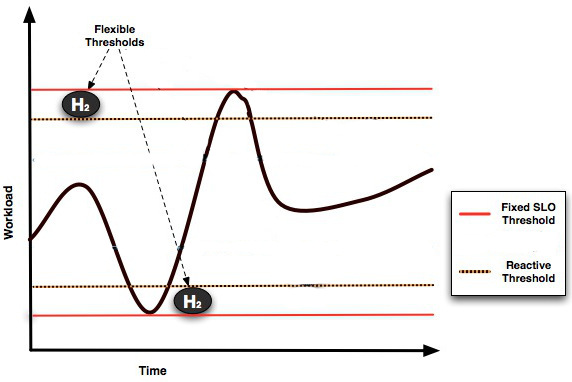
\includegraphics[width=.85\linewidth]{images/thresholdGraphic.jpg}
  \end{center}
\vspace{-5mm}
  \caption{Reactive Threshold.}
  \label{threshold}
\end{figure}

The scaling process starts by removing the noise from the monitoring data. Next the Scaler evaluates whether the current performance behavior requires to trigger any of the following scaling actions:

\begin{itemize}

\item \textbf{Scale out or up:} Additional resources are provisioned if the performance behavior exceeds the upper boundary of the reactive threshold, and the Predictor confirms that such traffic spike will remain at least during the next 5min. 

\item \textbf{Scale back or down:} Resources are released if the performance behaviour exceeds the lower boundary of the reactive threshold, and the Predictor confirms that such traffic oscillation will remain at least during the next 5min.

\end{itemize}

Note that, short-term (5min) forecasts operations are triggered to minimize at the maximum the number of SLA violations, as well as to keep a high level of efficiency in the predictions. 


\begin{figure*}[htb]
	\begin{minipage}[b]{0.3\linewidth}
		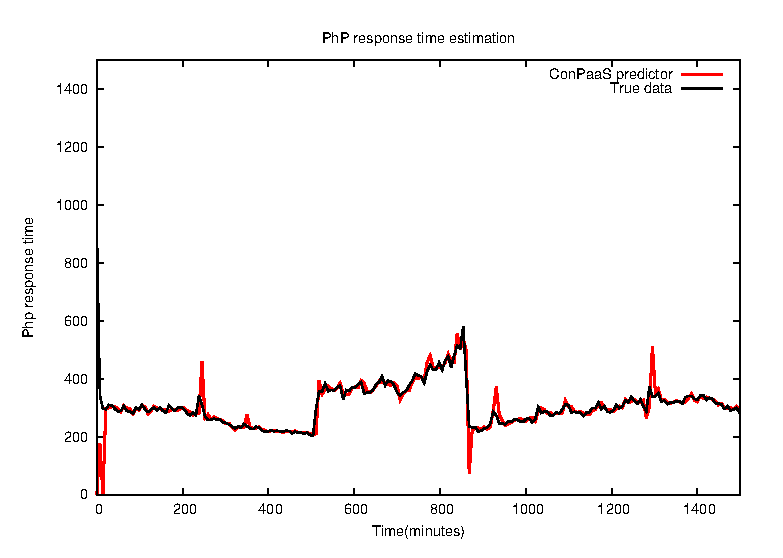
\includegraphics[height=4.5cm]{images/prediction_conpaas_6min.eps}
		\vspace{-4mm}
	\end{minipage}
	\hfill
	\begin{minipage}[b]{0.3\linewidth}
		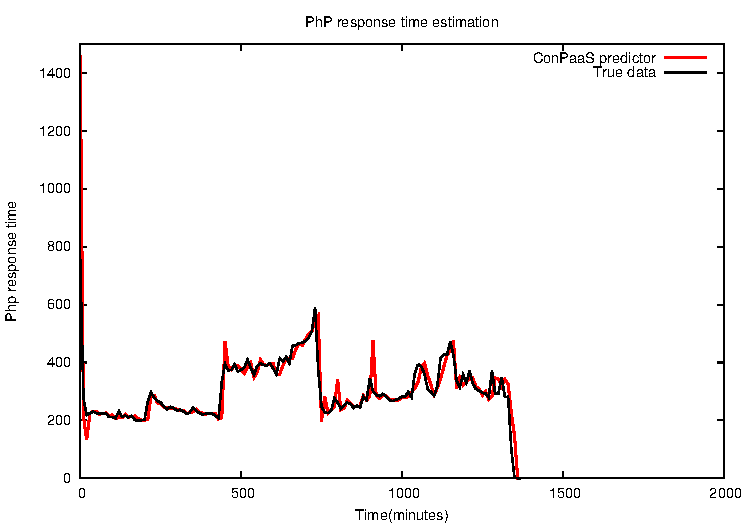
\includegraphics[height=4.5cm]{images/prediction_conpaas_10min}
		\vspace{-4mm}
	\end{minipage}
	\hfill
	\begin{minipage}[b]{0.3\linewidth}
		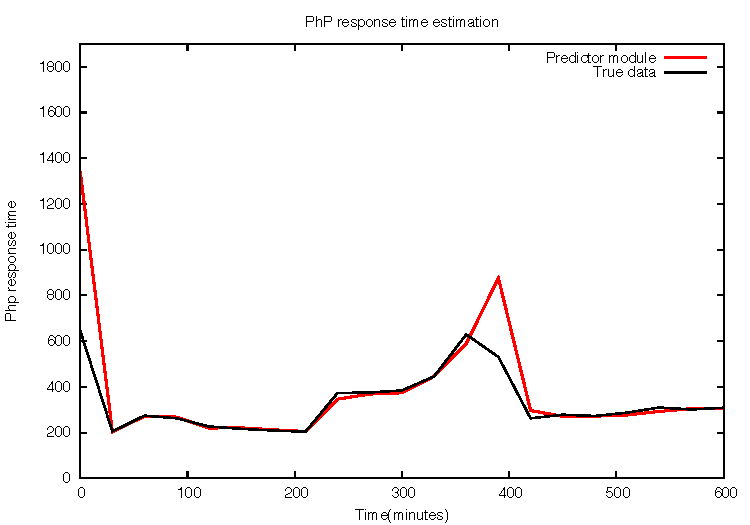
\includegraphics[height=4.5cm]{images/prediction_conpaas_30min}
		\vspace{-4mm}
	\end{minipage}
\caption{ConPaaS Predictor, response times for 5min, 10min and 30min ahead.}
\label{fig:vm_performance}
\end{figure*}

To decide which type of VM instances to release or add, the Scaler uses an optimal decision tree that calculates all the possible scaling strategies. In this decision tree, each node represents each type of VM instance provided by the cloud providers. The links indicate the percentage of CPU usage consumed to process the current workload when using a specific combination of nodes. To calculate the different combinations of VM instances that enforce the performance requirements, we used the next formula:

{\scriptsize
\begin{equation}\label{cpu_usage}
\begin{split}
CPU_{total} \geqslant \dfrac{ \sum_{i=1}^n ( \dfrac{ N\_reqs_{total} * Workload_{complex} }  {Num\_machines}  ) * CPU speed_{i} }  {Num\_machines} 
\end{split}
\end{equation}
}

In Equation~\ref{cpu_usage}, the \emph{$Workload_{complex}$} factor represents the complexity of the incoming traffic  which englobes effects such as those caused by the \emph{i.e.} operative system activities, vm sharing or request heterogeneity. $CPU_{total}$ and $N\_reqs_{total}$ are calculated by the Predictor component that estimates the future service demand for the next 30min (request rate and cpu usage). As illustrated in Figure~\ref{}, forecast operations of the resource requirements for the next 30min offer an aceptable level of accuracy. $CPU_{speed}$ is calculated using the Profiler component and will variate depending on the type of vm instance used in a strategy. The Equation~\ref{cpu_usage} answers to the question "How much and which type of vm instances to provision?".

Once the Scaler obtains a list of possible scaling strategies, they are classified based on their infrastructure cost and degree of slo fulfillment, as defined in the Equation~\ref{strategy_cost}. The infrastructure cost specifies the price required to provision extra cloud resources. While the slo fulfillment (slo\_cost in the Equation~\ref{strategy_cost}) represents the degree of vulnerability of a strategy to experience SLO violations. It is calculated based on the percentage of CPU usage of a strategy in comparison with the maximum CPU usage (based on the Amazon EC2 recomendations 75\%), and multiply by a SLO penalty (user pre-defined value). Obviously, higher values in the percentage of CPU usage imply an increment in the probabilty of having SLO violations, so slo\_cost will increase as well.


\begin{equation}\label{strategy_cost}
\begin{split}
slo\_cost =  ( \dfrac{ capacity } {max capacity} ) * slo penalty \\
cost\_strategy = \dfrac{  slo\_fulfillment  } {infra\_cost}
\end{split}
\end{equation}


Note that, the search of an optimal scaling strategy can represent a NP hard problem, so that we again used the CPU fixed threshold to limit the maximum or minimum CPU percentage value offered for a strategy. This assumption avoids to trigger new scaling actions in the next time interval saving costs.  Moreover, a cost policy was also included for avoiding to choose wasteful scaling strategies. This policy reject strategies releasing VM instances which have been recently started ( 5 < time to the end of its hour < 20). 

As explained in the Equation~\ref{strategy_cost}, the cost of a strategy is based on the cost incurred by its slo fulfillment degree and the infrastructure cost. To refine the search process with the goal of selecting the most appropriate strategy. Scaler provides three type classes of SLA agreements in function of the type of customer. The three classes of customers namely, gold, silver and bronze minimize the SLA violations with a different cost. Accordingly, a gold customer pays more in order to get the best service at the cost of some extra over-provisioning (lower slo cost). A silver customer gets good availability while a bronze customer obtains a reduced,
but acceptable, SLA fulfillment but with very little over-provisioning.

A complete point of view of the whole scaling flow is shown in Figure~\ref{autoScalingFlow}.

\begin{figure}[htb]
  \begin{center}
    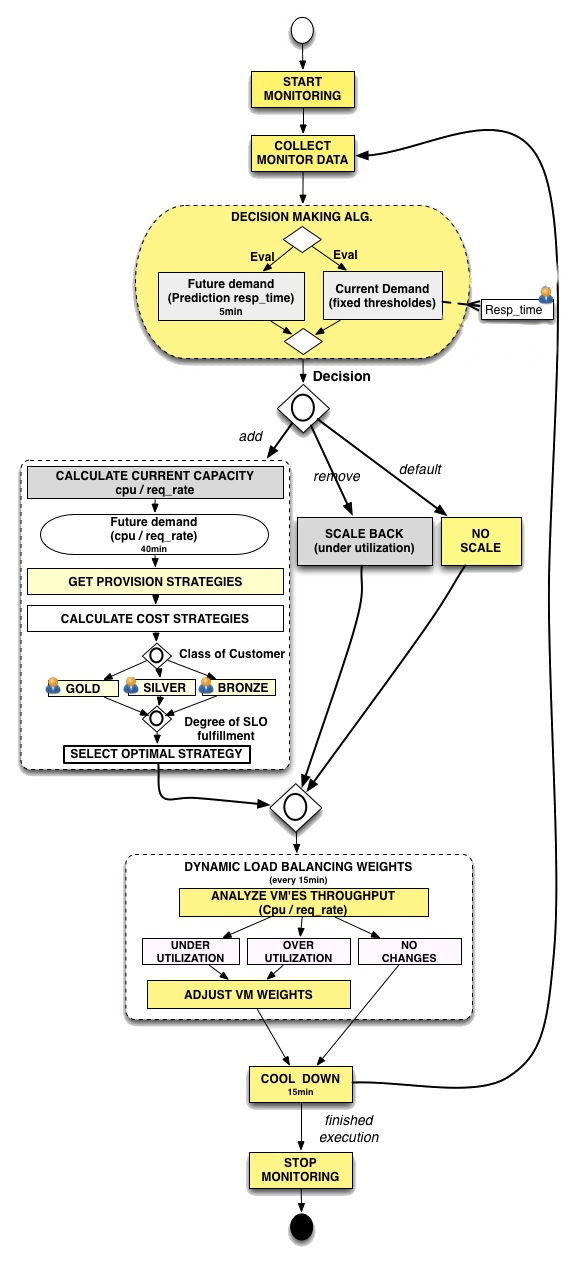
\includegraphics[width=\linewidth]{images/NewAutoScalingFlow}
  \end{center}
\vspace{-5mm}
  \caption{Auto scaling flow.}
  \label{autoScalingFlow}
\end{figure}


\subsection{Dynamic load balancing weights: } 

The problem we consider here is the heterogeneity of cloud platforms.
Different virtual machines from the same cloud might have different performance
characteristics, even when their specifications from the cloud vendor are 
the same~\cite{ec2Performance}. This issue can be addressed through various 
load balancing techniques, like assigning weights to the backend servers or 
taking into account the current number of connections that each server 
handles. Furthermore, the performance behavior of the virtual servers may 
also fluctuate, either due to changes in the application's usage 
patterns, or due to changes related to the hosting of the virtual servers 
(e.g., VM migration).

In order to address these issues in ConPaaS we implemented a weighted 
load balancing system in which the weights of the servers are 
periodically re-adjusted automatically, based on the monitoring data.  
This method assigns the same weight to each backend server at the 
beginning of the process. The weights are then periodically
adjusted (in our experiments, every $\sim$ 15min) proportionally 
with the difference among the average cpu\_usage and request rate of the servers 
during this time interval. By adding this technique to the feedback-based
algorithm, we noticed a performance improvement when running the
benchmarks, as discussed in the following.



